% This LaTeX document needs to be compiled with XeLaTeX.
\documentclass[10pt]{article}
\usepackage[utf8]{inputenc}
\usepackage{graphicx}
\usepackage[export]{adjustbox}
\graphicspath{ {./images/} }
\usepackage{amsmath}
\usepackage{amsfonts}
\usepackage{amssymb}
\usepackage[version=4]{mhchem}
\usepackage{stmaryrd}
\usepackage{multirow}
\usepackage[fallback]{xeCJK}
\usepackage{polyglossia}
\usepackage{fontspec}
\setCJKmainfont{Noto Serif CJK TC}

\setmainlanguage{polish}
\setmainfont{CMU Serif}

\title{EGZAMIN MATURALNY Z MATEMATYKI }

\author{}
\date{}


\begin{document}
\maketitle
\begin{center}
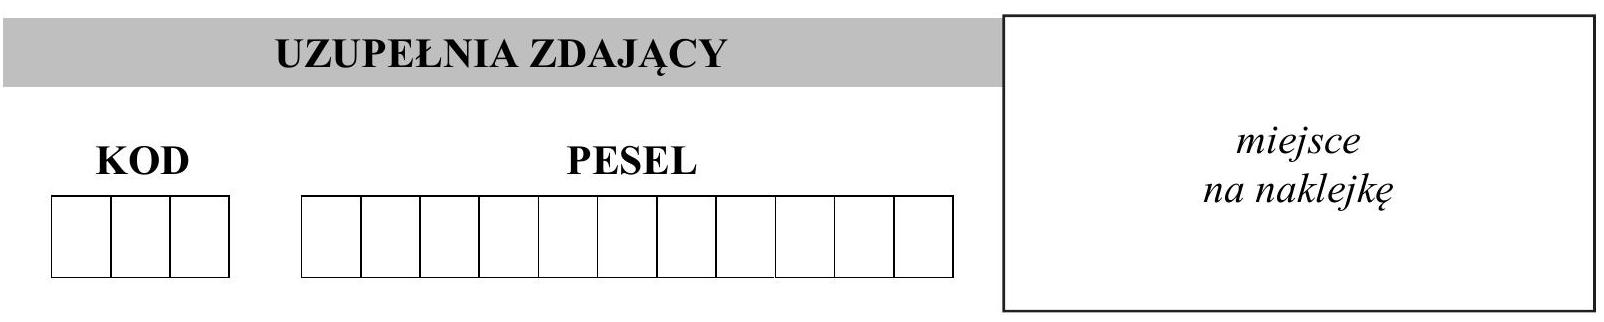
\includegraphics[max width=\textwidth]{2024_11_21_21760be7bf17f3e271c1g-01(1)}
\end{center}

Poziom ROZSZERZONY

Data:9 maja 2018 r. Godzina rozpoczęcia: 9:00\\
CZas pRAcy: \(\mathbf{1 8 0}\) minut\\
LICZBA PUNKTÓW DO UZYSKANIA: \(\mathbf{5 0}\)

\begin{center}
\begin{tabular}{|c|}
\hline
UZUPELNIA ZESPÓL \\
NADZORUJĄCY \\
\hline
Uprawnienia zdającego do: \\
\(\square \quad\)\begin{tabular}{l}
dostosowania \\
kryteriów oceniania \\
nieprzenoszenia \\
zaznaczeń na kartę \\
\end{tabular} \\
\hline
\end{tabular}
\end{center}

\section*{Instrukcja dla zdającego}
\begin{enumerate}
  \item Sprawdź, czy arkusz egzaminacyjny zawiera 18 stron (zadania 1-15). Ewentualny brak zgłoś przewodniczącemu zespołu nadzorującego egzamin.
  \item Rozwiązania zadań i odpowiedzi wpisuj w miejscu na to przeznaczonym.
  \item Odpowiedzi do zadań zamkniętych (1-4) zaznacz na karcie odpowiedzi w części karty przeznaczonej dla zdającego. Zamaluj \(\square\) pola do tego przeznaczone. Błędne zaznaczenie otocz kółkiem \({ }^{\text {i zaznacz właściwe. }}\)
  \item W zadaniu 5. wpisz odpowiednie cyfry w kratki pod treścią zadania.
  \item Pamiętaj, że pominięcie argumentacji lub istotnych obliczeń w rozwiązaniu zadania otwartego (6-15) może spowodować, że za to rozwiązanie nie otrzymasz pełnej liczby punktów.
  \item Pisz czytelnie i używaj tylko długopisu lub pióra z czarnym tuszem lub atramentem.
  \item Nie używaj korektora, a błędne zapisy wyraźnie przekreśl.
  \item Pamiętaj, że zapisy w brudnopisie nie będą oceniane.
  \item Możesz korzystać z zestawu wzorów matematycznych, cyrkla i linijki oraz kalkulatora prostego.
  \item Na tej stronie oraz na karcie odpowiedzi wpisz swój numer PESEL i przyklej naklejkę z kodem.
  \item Nie wpisuj żadnych znaków w części przeznaczonej dla egzaminatora.\\

\includegraphics[max width=\textwidth, center]{2024_11_21_21760be7bf17f3e271c1g-01}
\end{enumerate}

W zadaniach od 1. do 4. wybierz i zaznacz na karcie odpowiedzi poprawna odpowiedź.

\section*{Zadanie 1. (0-1)}
Dane są liczby: \(a=\frac{\sqrt[4]{8}}{2}, b=\frac{1}{2 \sqrt[4]{8}}, c=\sqrt[4]{8}, d=\frac{2}{\sqrt[4]{8}}\) oraz \(k=2^{-\frac{1}{4}}\). Prawdziwa jest równość\\
A. \(k=a\)\\
B. \(k=b\)\\
C. \(k=c\)\\
D. \(k=d\)

\section*{Zadanie 2. (0-1)}
Równanie \(||x|-2|=|x|+2\)\\
A. nie ma rozwiązań.\\
B. ma dokładnie jedno rozwiązanie.\\
C. ma dokładnie dwa rozwiązania.\\
D. ma dokładnie cztery rozwiązania.

\section*{Zadanie 3. (0-1)}
Wartość wyrażenia \(2 \log _{5} 10-\frac{1}{\log _{20} 5}\) jest równa\\
A. -1\\
B. 0\\
C. 1\\
D. 2

\section*{Zadanie 4. (0-1)}
Granica \(\lim _{x \rightarrow 3^{-}} \frac{-x+2}{x^{2}-5 x+6}\) jest równa\\
A. \(-\infty\)\\
B. -1\\
C. 0\\
D. \(+\infty\)

\section*{BRUDNOPIS (nie podlega ocenie)}
\begin{center}

\includegraphics[max width=\textwidth]{2024_11_21_21760be7bf17f3e271c1g-03}
\end{center}

\section*{Zadanie 5. (0-2)}
Punkt \(A=(-5,3)\) jest środkiem symetrii wykresu funkcji homograficznej określonej wzorem \(f(x)=\frac{a x+7}{x+d}\), gdy \(x \neq-d\). Oblicz iloraz \(\frac{d}{a}\).\\
W poniższe kratki wpisz kolejno cyfrę jedności i pierwsze dwie cyfry po przecinku nieskończonego rozwinięcia dziesiętnego otrzymanego wyniku.

\begin{center}
\begin{tabular}{|l|l|l|}
\hline
 &  &  \\
\hline
\end{tabular}
\end{center}

\section*{BRUDNOPIS (nie podlega ocenie)}
\begin{center}
\begin{tabular}{|c|c|c|c|c|c|c|c|c|c|c|c|c|c|c|c|c|c|c|c|c|c|c|c|}
\hline
 &  &  &  &  & 到 &  & 到 & - &  & - &  & - &  & - & - & - &  & - & - &  & - & | &  \\
\hline
 &  &  &  &  &  &  &  &  &  &  &  &  &  &  &  &  &  &  &  &  &  &  &  \\
\hline
 &  &  &  &  &  &  &  &  &  &  &  &  &  &  &  &  &  &  &  &  &  &  &  \\
\hline
 &  &  &  &  &  &  &  &  &  &  &  &  &  &  &  &  &  &  &  &  &  &  &  \\
\hline
 &  &  &  &  &  &  &  &  &  &  &  &  &  &  &  &  &  &  &  &  &  &  &  \\
\hline
 &  &  &  &  &  &  &  &  &  &  &  &  &  &  &  &  &  &  &  &  &  &  &  \\
\hline
 &  &  &  &  &  &  &  &  &  &  &  &  &  &  &  &  &  &  &  &  &  &  &  \\
\hline
 &  &  &  &  &  &  &  &  &  &  &  &  &  &  &  &  &  &  &  &  &  &  &  \\
\hline
 &  &  &  &  &  &  &  &  &  &  &  &  &  &  &  &  &  &  &  &  &  &  &  \\
\hline
 &  &  &  &  &  &  &  &  &  &  &  &  &  &  &  &  &  &  &  &  &  &  &  \\
\hline
 &  &  &  &  &  &  &  &  &  &  &  &  &  &  &  &  &  &  &  &  &  &  &  \\
\hline
 &  &  &  &  &  &  &  &  &  &  &  &  &  &  &  &  &  &  &  &  &  &  &  \\
\hline
\end{tabular}
\end{center}

\section*{Zadanie 6. (0-3)}
Styczna do paraboli o równaniu \(y=\sqrt{3} x^{2}-1\) w punkcie \(P=\left(x_{0}, y_{0}\right)\) jest nachylona do osi \(O x\) pod kątem \(30^{\circ}\). Oblicz współrzędne punktu \(P\).\\

\includegraphics[max width=\textwidth, center]{2024_11_21_21760be7bf17f3e271c1g-04}

Odpowiedź: \(\qquad\)

\section*{Zadanie 7. (0-3)}
Trójkąt \(A B C\) jest ostrokątny oraz \(|A C|>|B C|\). Dwusieczna \(d_{C}\) kąta \(A C B\) przecina bok \(A B\) w punkcie \(K\). Punkt \(L\) jest obrazem punktu \(K\) w symetrii osiowej względem dwusiecznej \(d_{A}\) kąta \(B A C\), punkt \(M\) jest obrazem punktu \(L\) w symetrii osiowej względem dwusiecznej \(d_{C}\) kąta \(A C B\), a punkt \(N\) jest obrazem punktu \(M\) w symetrii osiowej względem dwusiecznej \(d_{B}\) kąta \(A B C\) (zobacz rysunek).\\
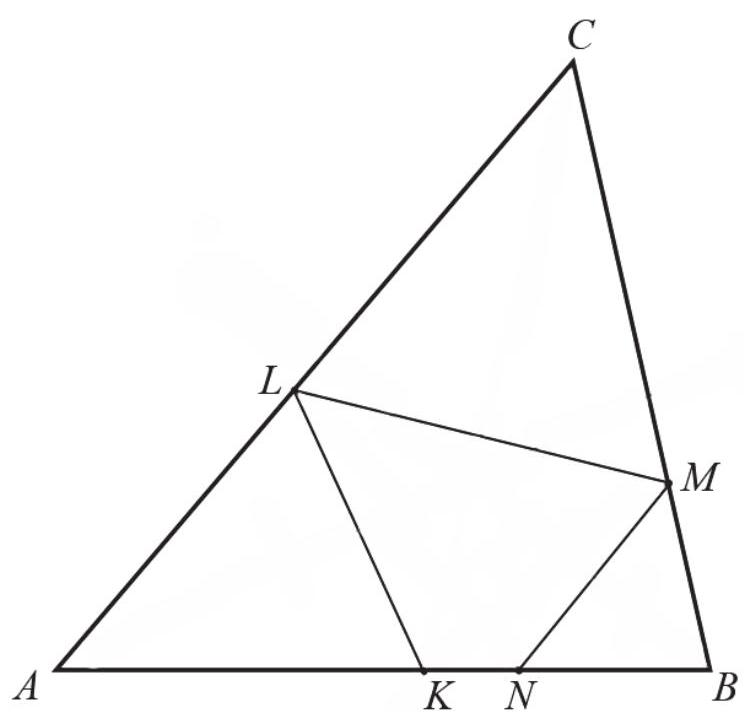
\includegraphics[max width=\textwidth, center]{2024_11_21_21760be7bf17f3e271c1g-05}

Udowodnij, że na czworokącie \(K N M L\) można opisać okrąg.\\

\includegraphics[max width=\textwidth, center]{2024_11_21_21760be7bf17f3e271c1g-05(1)}

\begin{center}
\begin{tabular}{|c|l|c|c|c|}
\hline
\multirow{2}{*}{\begin{tabular}{c}
Wypelnia \\
egzaminator \\
\end{tabular}} & Nr zadania & 5. & \(\mathbf{6 .}\) & \(\mathbf{7 .}\) \\
\cline { 2 - 5 }
 & Maks. liczba pkt & \(\mathbf{2}\) & \(\mathbf{3}\) & \(\mathbf{3}\) \\
\cline { 2 - 5 }
 & Uzyskana liczba pkt &  &  &  \\
\hline
\end{tabular}
\end{center}

\section*{Zadanie 8. (0-3)}
Udowodnij, że dla każdej liczby całkowitej \(k\) i dla każdej liczby całkowitej \(m\) liczba \(k^{3} m-k m^{3}\) jest podzielna przez 6.\\

\includegraphics[max width=\textwidth, center]{2024_11_21_21760be7bf17f3e271c1g-06}

\section*{Zadanie 9. (0-4)}
Z liczb ośmioelementowego zbioru \(Z=\{1,2,3,4,5,6,7,9\}\) tworzymy ośmiowyrazowy ciąg, którego wyrazy się nie powtarzają. Oblicz prawdopodobieństwo zdarzenia polegającego na tym, że żadne dwie liczby parzyste nie są sąsiednimi wyrazami utworzonego ciągu. Wynik przedstaw w postaci ułamka zwykłego nieskracalnego.\\

\includegraphics[max width=\textwidth, center]{2024_11_21_21760be7bf17f3e271c1g-07}

Odpowiedź:

\begin{center}
\begin{tabular}{|c|l|c|c|}
\hline
\multirow{3}{*}{\begin{tabular}{l}
Wypelnia \\
egzaminator \\
\end{tabular}} & Nr zadania & \(\mathbf{8 .}\) & \(\mathbf{9 .}\) \\
\cline { 2 - 4 }
 & Maks. liczba pkt & 3 & 4 \\
\cline { 2 - 4 }
 & Uzyskana liczba pkt &  &  \\
\hline
\end{tabular}
\end{center}

\section*{Zadanie 10. (0-4)}
Objętość stożka ściętego (przedstawionego na rysunku) można obliczyć ze wzoru \(V=\frac{1}{3} \pi H\left(r^{2}+r R+R^{2}\right)\), gdzie \(r\) i \(R\) są promieniami podstaw \((r<R)\), a \(H\) jest wysokością bryły. Dany jest stożek ścięty, którego wysokość jest równa 10, objętość \(840 \pi\), a \(r=6\). Oblicz cosinus kąta nachylenia przekątnej przekroju osiowego tej bryły do jednej z jej podstaw.\\
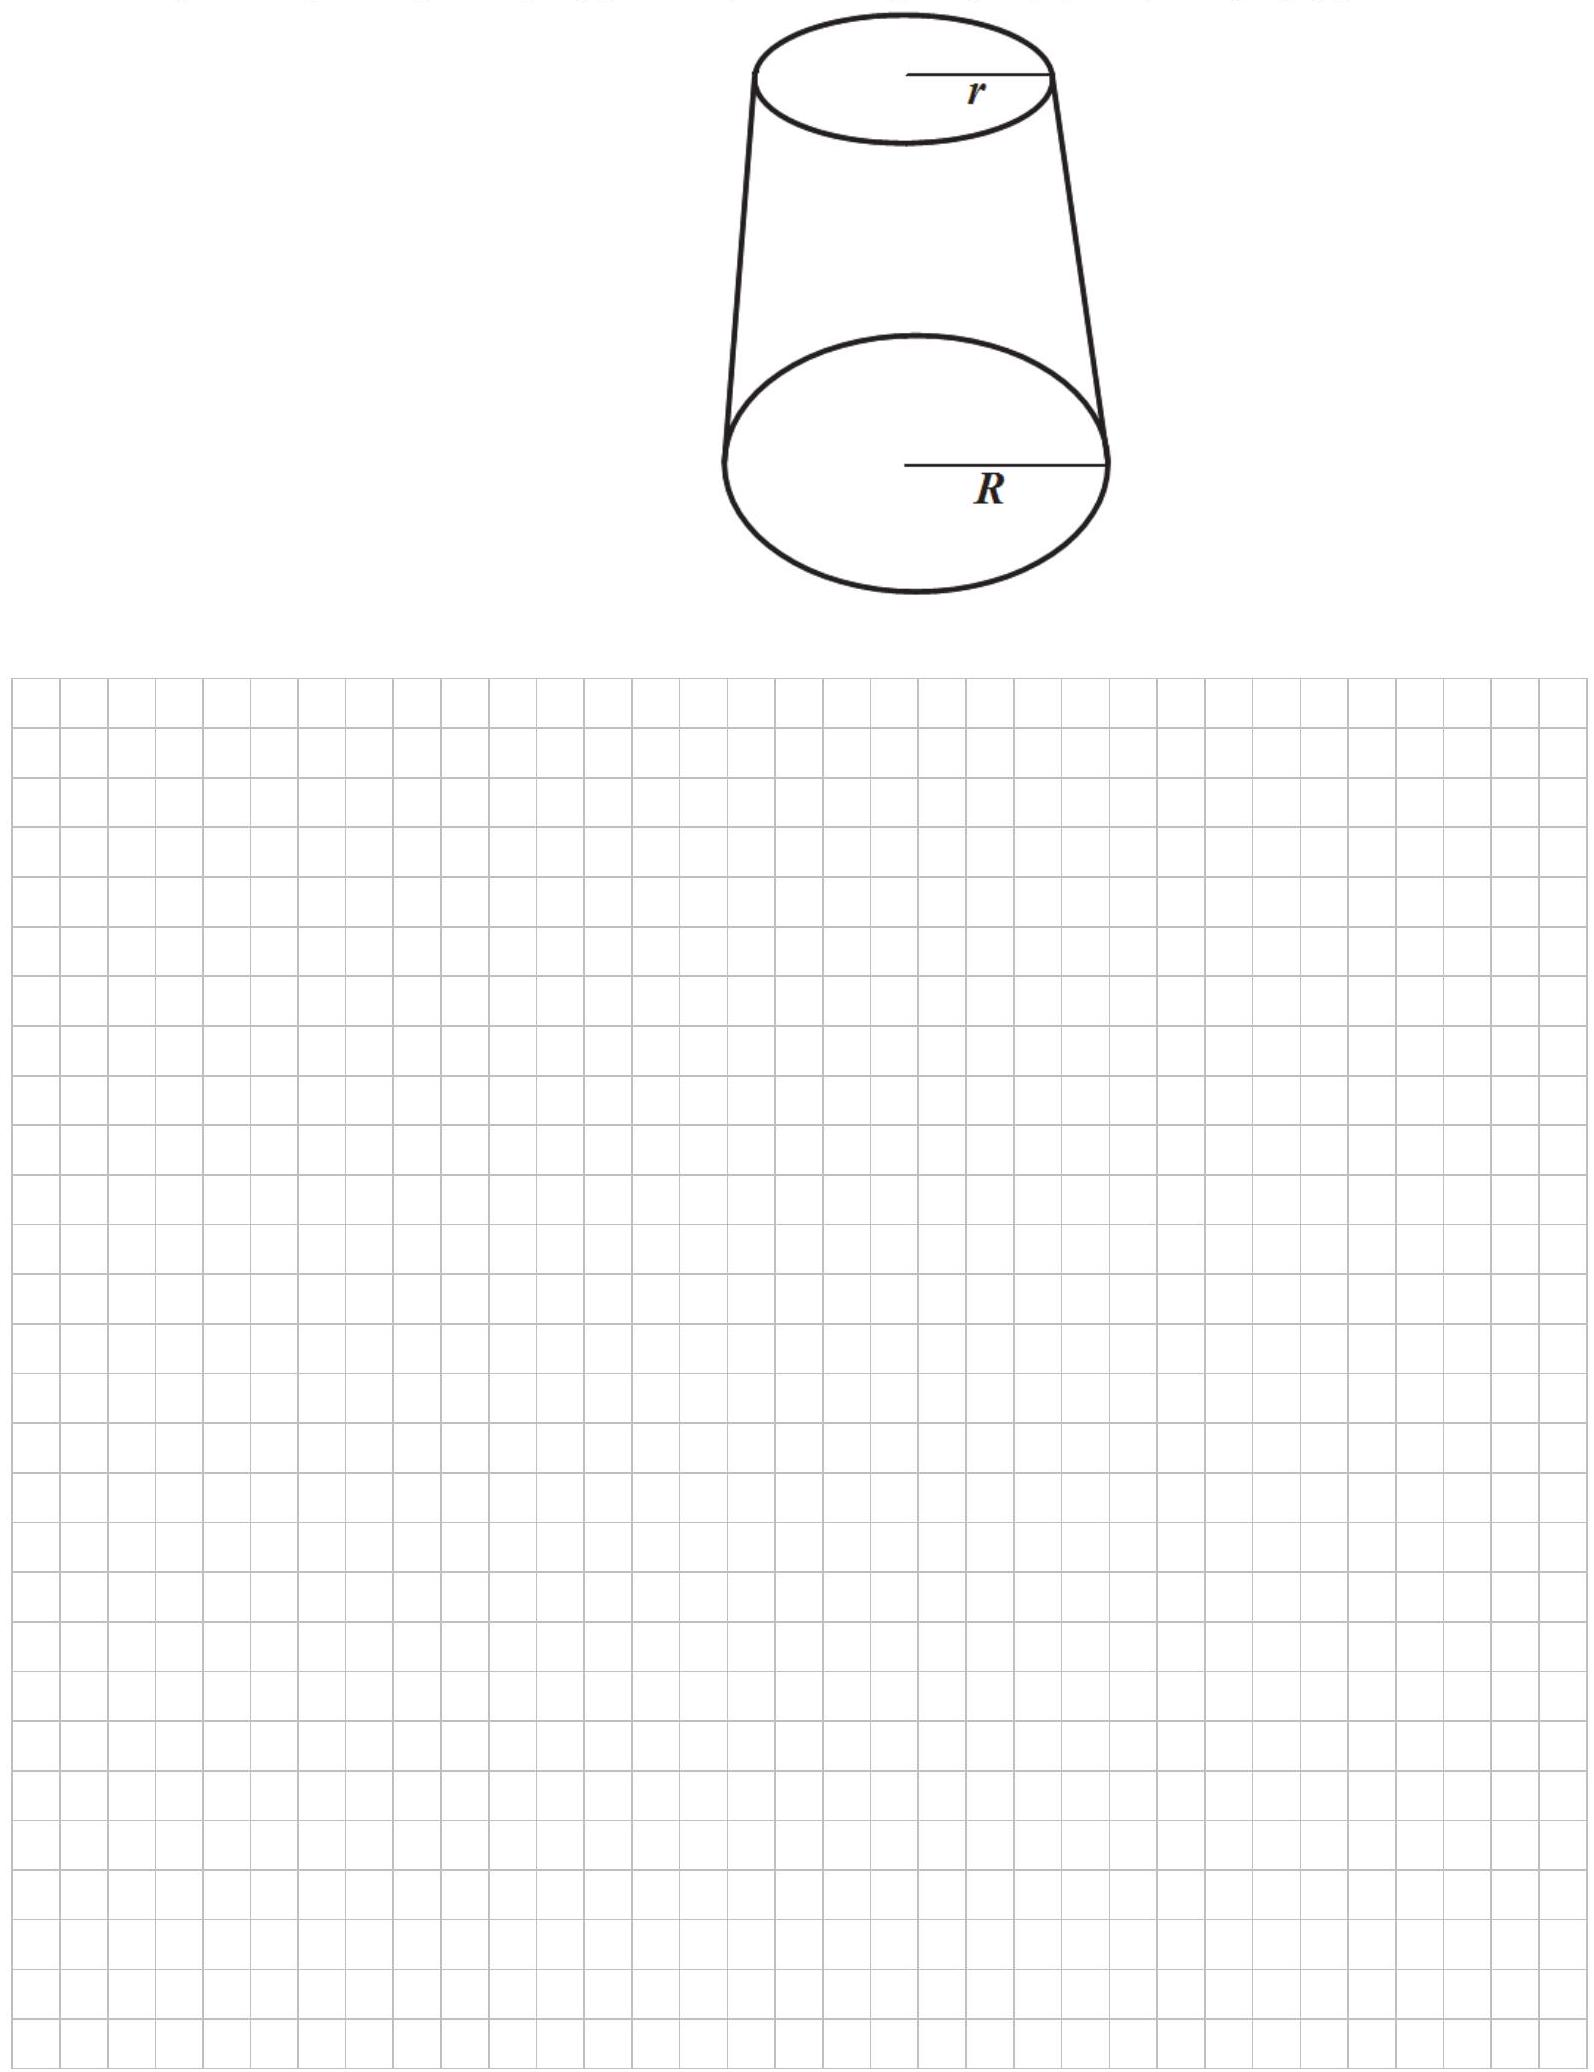
\includegraphics[max width=\textwidth, center]{2024_11_21_21760be7bf17f3e271c1g-08}

Odpowiedź: \(\qquad\)

\section*{Zadanie 11. (0-4)}
Rozwiąż równanie \(\sin 6 x+\cos 3 x=2 \sin 3 x+1 \mathrm{w}\) przedziale \(\langle 0, \pi\rangle\).\\

\includegraphics[max width=\textwidth, center]{2024_11_21_21760be7bf17f3e271c1g-09}

Odpowiedź:

\begin{center}
\begin{tabular}{|c|l|c|c|}
\hline
\multirow{3}{*}{\begin{tabular}{c}
Wypełnia \\
egzaminator \\
\end{tabular}} & Nr zadania & 10. & 11. \\
\cline { 2 - 4 }
 & Maks. liczba pkt & 4 & 4 \\
\cline { 2 - 4 }
 & Uzyskana liczba pkt &  &  \\
\hline
\end{tabular}
\end{center}

Zadanie 12. (0-6)\\
Wyznacz wszystkie wartości parametru \(m\), dla których równanie \(x^{2}+(m+1) x-m^{2}+1=0\) ma dwa rozwiązania rzeczywiste \(x_{1}\) i \(x_{2}\left(x_{1} \neq x_{2}\right)\), spełniające warunek \(x_{1}^{3}+x_{2}^{3}>-7 x_{1} x_{2}\).

\begin{center}
\begin{tabular}{|c|c|c|c|c|c|c|c|c|c|c|c|c|c|c|c|c|c|c|c|c|c|c|c|c|c|c|c|}
\hline
 &  &  &  &  &  &  &  &  &  &  &  &  &  &  &  &  &  &  &  &  &  &  &  &  &  &  &  \\
\hline
 &  &  &  &  &  &  &  &  &  &  &  &  &  &  &  &  &  &  &  &  &  &  &  &  &  &  &  \\
\hline
 &  &  &  &  &  &  &  &  &  &  &  &  &  &  &  &  &  &  &  &  &  &  &  &  &  &  &  \\
\hline
 &  &  &  &  &  &  &  &  &  &  &  &  &  &  &  &  &  &  &  &  &  &  &  &  &  &  &  \\
\hline
 &  &  &  &  &  &  &  &  &  &  &  &  &  &  &  &  &  &  &  &  &  &  &  &  &  &  &  \\
\hline
 &  &  &  &  &  &  &  &  &  &  &  &  &  &  &  &  &  &  &  &  &  &  &  &  &  &  &  \\
\hline
 &  &  &  &  &  &  &  &  &  &  &  &  &  &  &  &  &  &  &  &  &  &  &  &  &  &  &  \\
\hline
 &  &  &  &  &  &  &  &  &  &  &  &  &  &  &  &  &  &  &  &  &  &  &  &  &  &  &  \\
\hline
 &  &  &  &  &  &  &  &  &  &  &  &  &  &  &  &  &  &  &  &  &  &  &  &  &  &  &  \\
\hline
 &  &  &  &  &  &  &  &  &  &  &  &  &  &  &  &  &  &  &  &  &  &  &  &  &  &  &  \\
\hline
 &  &  &  &  &  &  &  &  &  &  &  &  &  &  &  &  &  &  &  &  &  &  &  &  &  &  &  \\
\hline
 &  &  &  &  &  &  &  &  &  &  &  &  &  &  &  &  &  &  &  &  &  &  &  &  &  &  &  \\
\hline
 &  &  &  &  &  &  &  &  &  &  &  &  &  &  &  &  &  &  &  &  &  &  &  &  &  &  &  \\
\hline
 &  &  &  &  &  &  &  &  &  &  &  &  &  &  &  &  &  &  &  &  &  &  &  &  &  &  &  \\
\hline
 &  &  &  &  &  &  &  &  &  &  &  &  &  &  &  &  &  &  &  &  &  &  &  &  &  &  &  \\
\hline
 &  &  &  &  &  &  &  &  &  &  &  &  &  &  &  &  &  &  &  &  &  &  &  &  &  &  &  \\
\hline
 &  &  &  &  &  &  &  &  &  &  &  &  &  &  &  &  &  &  &  &  &  &  &  &  &  &  &  \\
\hline
 &  &  &  &  &  &  &  &  &  &  &  &  &  &  &  &  &  &  &  &  &  &  &  &  &  &  &  \\
\hline
 &  &  &  &  &  &  &  &  &  &  &  &  &  &  &  &  &  &  &  &  &  &  &  &  &  &  &  \\
\hline
 &  &  &  &  &  &  &  &  &  &  &  &  &  &  &  &  &  &  &  &  &  &  &  &  &  &  &  \\
\hline
 &  &  &  &  &  &  &  &  &  &  &  &  &  &  &  &  &  &  &  &  &  &  &  &  &  &  &  \\
\hline
 &  &  &  &  &  &  &  &  &  &  &  &  &  &  &  &  &  &  &  &  &  &  &  &  &  &  &  \\
\hline
 &  &  &  &  &  &  &  &  &  &  &  &  &  &  &  &  &  &  &  &  &  &  &  &  &  &  &  \\
\hline
 &  &  &  &  &  &  &  &  &  &  &  &  &  &  &  &  &  &  &  &  &  &  &  &  &  &  &  \\
\hline
 &  &  &  &  &  &  &  &  &  &  &  &  &  &  &  &  &  &  &  &  &  &  &  &  &  &  &  \\
\hline
 &  &  &  &  &  &  &  &  &  &  &  &  &  &  &  &  &  &  &  &  &  &  &  &  &  &  &  \\
\hline
 &  &  &  &  &  &  &  &  &  &  &  &  &  &  &  &  &  &  &  &  &  &  &  &  &  &  &  \\
\hline
 &  &  &  &  &  &  &  &  &  &  &  &  &  &  &  &  &  &  &  &  &  &  &  &  &  &  &  \\
\hline
 &  &  &  &  &  &  &  &  &  &  &  &  &  &  &  &  &  &  &  &  &  &  &  &  &  & 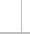
\includegraphics[max width=\textwidth]{2024_11_21_21760be7bf17f3e271c1g-10(1)}
 &  \\
\hline
 &  &  &  &  &  &  &  &  &  &  &  &  &  &  &  &  &  &  &  &  &  &  &  &  &  &  &  \\
\hline
 &  &  &  &  &  &  &  &  &  &  &  &  &  &  &  &  &  &  &  &  &  &  &  &  &  &  &  \\
\hline
 & 
\includegraphics[max width=\textwidth]{2024_11_21_21760be7bf17f3e271c1g-10(3)}
 &  &  &  &  &  &  &  &  &  &  &  &  &  &  &  &  &  &  &  &  &  &  &  &  &  &  \\
\hline
 & 
\includegraphics[max width=\textwidth]{2024_11_21_21760be7bf17f3e271c1g-10}
 &  &  &  &  &  &  &  &  &  &  &  &  &  &  &  &  &  &  &  &  &  &  &  &  &  &  \\
\hline
 &  &  &  &  &  &  &  &  &  &  &  &  &  &  &  &  &  &  &  &  &  &  &  &  &  &  &  \\
\hline
 &  &  &  &  &  &  &  &  &  &  &  &  &  &  &  &  &  &  &  &  &  &  &  &  &  &  &  \\
\hline
 &  &  &  &  &  &  &  &  &  &  &  &  &  &  &  &  &  &  &  &  &  &  &  &  &  &  &  \\
\hline
 &  &  &  &  &  &  &  &  &  &  &  &  &  &  &  &  &  &  &  &  &  &  &  &  &  &  &  \\
\hline
 &  &  &  &  &  &  &  &  &  &  &  &  &  &  &  &  &  &  &  &  &  &  &  &  &  &  &  \\
\hline
 &  &  &  &  &  &  &  &  &  &  &  &  &  &  &  &  &  &  &  &  &  &  &  &  &  & 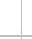
\includegraphics[max width=\textwidth]{2024_11_21_21760be7bf17f3e271c1g-10(2)}
 &  \\
\hline
 &  &  &  &  &  &  &  &  &  &  &  &  &  &  &  &  &  &  &  &  &  &  &  &  &  &  &  \\
\hline
 &  &  &  &  &  &  &  &  &  &  &  &  &  &  &  &  &  &  &  &  &  &  &  &  &  &  &  \\
\hline
 &  &  &  &  &  &  &  &  &  &  &  &  &  &  &  &  &  &  &  &  &  &  &  &  &  &  &  \\
\hline
 &  &  &  &  &  &  &  &  &  &  &  &  &  &  &  &  &  &  &  &  &  &  &  &  &  &  &  \\
\hline
 &  &  &  &  &  &  &  &  &  &  &  &  &  &  &  &  &  &  &  &  &  &  &  &  &  &  &  \\
\hline
 &  &  &  &  &  &  &  &  &  &  &  &  &  &  &  &  &  &  &  &  &  &  &  &  &  &  &  \\
\hline
\end{tabular}
\end{center}

\begin{center}

\includegraphics[max width=\textwidth]{2024_11_21_21760be7bf17f3e271c1g-11}
\end{center}

Odpowiedź: \(\qquad\)

\begin{center}
\begin{tabular}{|c|l|c|}
\hline
\multirow{2}{*}{\begin{tabular}{c}
Wypelnia \\
egzaminator \\
\end{tabular}} & Nr zadania & 12. \\
\cline { 2 - 3 }
 & Maks. liczba pkt & 6 \\
\cline { 2 - 3 }
 & Uzyskana liczba pkt &  \\
\hline
\end{tabular}
\end{center}

\section*{Zadanie 13. (0-4)}
Wyrazy ciągu geometrycznego \(\left(a_{n}\right)\), określonego dla \(n \geq 1\), spełniają układ równań

\[
\left\{\begin{array}{l}
a_{3}+a_{6}=-84 \\
a_{4}+a_{7}=168
\end{array}\right.
\]

Wyznacz liczbę \(n\) początkowych wyrazów tego ciągu, których suma \(S_{n}\) jest równa 32769.

\begin{center}
\begin{tabular}{|c|c|c|c|c|c|c|c|c|c|c|c|c|c|c|c|c|c|c|c|c|c|c|}
\hline
 &  &  &  &  &  &  &  &  &  &  &  &  &  &  &  &  &  &  &  &  &  &  \\
\hline
 &  &  &  &  &  &  &  &  &  &  &  &  &  &  &  &  &  &  &  &  &  &  \\
\hline
 &  &  &  &  &  &  &  &  &  &  &  &  &  &  &  &  &  &  &  &  &  &  \\
\hline
 &  &  &  &  &  &  &  &  &  &  &  &  &  &  &  &  &  &  &  &  &  &  \\
\hline
 &  &  &  &  &  &  &  &  &  &  &  &  &  &  &  &  &  &  &  &  &  &  \\
\hline
 &  &  &  &  &  &  &  &  &  &  &  &  &  &  &  &  &  &  &  &  &  &  \\
\hline
 &  &  &  &  &  &  &  &  &  &  &  &  &  &  &  &  &  &  &  &  &  &  \\
\hline
 &  &  &  &  &  &  &  &  &  &  &  &  &  &  &  &  &  &  &  &  &  &  \\
\hline
 &  &  &  &  &  &  &  &  &  &  &  &  &  &  &  &  &  &  &  &  &  &  \\
\hline
 &  &  &  &  &  &  &  &  &  &  &  &  &  &  &  &  &  &  &  &  &  &  \\
\hline
 &  &  &  &  &  &  &  &  &  &  &  &  &  &  &  &  &  &  &  &  &  &  \\
\hline
 &  &  &  &  &  &  &  &  &  &  &  &  &  &  &  &  &  &  &  &  &  &  \\
\hline
 &  &  &  &  &  &  &  &  &  &  &  &  &  &  &  &  &  &  &  &  &  &  \\
\hline
 &  &  &  &  &  &  &  &  &  &  &  &  &  &  &  &  &  &  &  &  &  &  \\
\hline
 &  &  &  &  &  &  &  &  &  &  &  &  &  &  &  &  &  &  &  &  &  &  \\
\hline
 &  &  &  &  &  &  &  &  &  &  &  &  &  &  &  &  &  &  &  &  &  &  \\
\hline
 &  &  &  &  &  &  &  &  &  &  &  &  &  &  &  &  &  &  &  &  &  &  \\
\hline
 &  &  &  &  &  &  &  &  &  &  &  &  &  &  &  &  &  &  &  &  &  &  \\
\hline
 &  &  &  &  &  &  &  &  &  &  &  &  &  &  &  &  &  &  &  &  &  &  \\
\hline
 &  &  &  &  &  &  &  &  &  &  &  &  &  &  &  &  &  &  &  &  &  &  \\
\hline
 &  &  &  &  &  &  &  &  &  &  &  &  &  &  &  &  &  &  &  &  &  &  \\
\hline
 &  &  &  &  &  &  &  &  &  &  &  &  &  &  &  &  &  &  &  &  &  &  \\
\hline
 &  &  &  &  &  &  &  &  &  &  &  &  &  &  &  &  &  &  &  &  &  &  \\
\hline
 &  &  &  &  &  &  &  &  &  &  &  &  &  &  &  &  &  &  &  &  &  &  \\
\hline
 &  &  &  &  &  &  &  &  &  &  &  &  &  &  &  &  &  &  &  &  &  &  \\
\hline
 &  &  &  &  &  &  &  &  &  &  &  &  &  &  &  &  &  &  &  &  &  &  \\
\hline
 &  &  &  &  &  &  &  &  &  &  &  &  &  &  &  &  &  &  &  &  &  &  \\
\hline
 &  &  &  &  &  &  &  &  &  &  &  &  &  &  &  &  &  &  &  &  &  &  \\
\hline
 &  &  &  &  &  &  &  &  &  &  &  &  &  &  &  &  &  &  &  &  &  &  \\
\hline
 &  &  &  &  &  &  &  &  &  &  &  &  &  &  &  &  &  &  &  &  &  &  \\
\hline
 &  &  &  &  &  &  &  &  &  &  &  &  &  &  &  &  &  &  &  &  &  &  \\
\hline
 &  &  &  &  &  &  &  &  &  &  &  &  &  &  &  &  &  &  &  &  &  &  \\
\hline
 &  &  &  &  &  &  &  &  &  &  &  &  &  &  &  &  &  &  &  &  &  &  \\
\hline
 &  &  &  &  &  &  &  &  &  &  &  &  &  &  &  &  &  &  &  &  &  &  \\
\hline
 &  &  &  &  &  &  &  &  &  &  &  &  &  &  &  &  &  &  &  &  &  &  \\
\hline
 &  &  &  &  &  &  &  &  &  &  &  &  &  &  &  &  &  &  &  &  &  &  \\
\hline
 &  &  &  &  &  &  &  &  &  &  &  &  &  &  &  &  &  &  &  &  &  &  \\
\hline
 &  &  &  &  &  &  &  &  &  &  &  &  &  &  &  &  &  &  &  &  &  &  \\
\hline
 &  &  &  &  &  &  &  &  &  &  &  &  &  &  &  &  &  &  &  &  &  &  \\
\hline
 &  &  &  &  &  &  &  &  &  &  &  &  &  &  &  &  &  &  &  &  &  &  \\
\hline
 &  &  &  &  &  &  &  &  &  &  &  &  &  &  &  &  &  &  &  &  &  &  \\
\hline
 &  &  &  &  &  &  &  &  &  &  &  &  &  &  &  &  &  &  &  &  &  &  \\
\hline
 &  &  &  &  &  &  &  &  &  &  &  &  &  &  &  &  &  &  &  &  &  &  \\
\hline
\end{tabular}
\end{center}

\begin{center}

\includegraphics[max width=\textwidth]{2024_11_21_21760be7bf17f3e271c1g-13}
\end{center}

Odpowiedź: \(\qquad\)

\begin{center}
\begin{tabular}{|c|l|c|}
\hline
\multirow{2}{*}{\begin{tabular}{c}
Wypelnia \\
egzaminator \\
\end{tabular}} & Nr zadania & 13. \\
\cline { 2 - 3 }
 & Maks. liczba pkt & 4 \\
\cline { 2 - 3 }
 & Uzyskana liczba pkt &  \\
\hline
\end{tabular}
\end{center}

\section*{Zadanie 14. (0-6)}
Punkt \(A=(7,-1)\) jest wierzchołkiem trójkąta równoramiennego \(A B C\), w którym \(|A C|=|B C|\). Obie współrzędne wierzchołka \(C\) są liczbami ujemnymi. Okrąg wpisany w trójkąt \(A B C\) ma równanie \(x^{2}+y^{2}=10\). Oblicz współrzędne wierzchołków \(B\) i \(C\) tego trójkąta.\\

\includegraphics[max width=\textwidth, center]{2024_11_21_21760be7bf17f3e271c1g-14}\\

\includegraphics[max width=\textwidth, center]{2024_11_21_21760be7bf17f3e271c1g-15}

Odpowiedź:

\begin{center}
\begin{tabular}{|c|l|c|}
\hline
\multirow{2}{*}{\begin{tabular}{l}
Wypelnia \\
egzaminator \\
\end{tabular}} & Nr zadania & 14. \\
\cline { 2 - 3 }
 & Maks. liczba pkt & 6 \\
\cline { 2 - 3 }
 & Uzyskana liczba pkt &  \\
\hline
\end{tabular}
\end{center}

\section*{Zadanie 15. (0-7)}
Rozpatrujemy wszystkie trapezy równoramienne, w które można wpisać okrąg, spełniające warunek: suma długości dłuższej podstawy \(a\) i wysokości trapezu jest równa 2.\\
a) Wyznacz wszystkie wartości \(a\), dla których istnieje trapez o podanych własnościach.\\
b) Wykaż, że obwód \(L\) takiego trapezu, jako funkcja długości \(a\) dłuższej podstawy trapezu, wyraża się wzorem \(L(a)=\frac{4 a^{2}-8 a+8}{a}\).\\
c) Oblicz tangens kąta ostrego tego spośród rozpatrywanych trapezów, którego obwód jest najmniejszy.\\

\includegraphics[max width=\textwidth, center]{2024_11_21_21760be7bf17f3e271c1g-16}\\

\includegraphics[max width=\textwidth, center]{2024_11_21_21760be7bf17f3e271c1g-17}

Odpowiedź: \(\qquad\)

\begin{center}
\begin{tabular}{|c|l|c|}
\hline
\multirow{2}{*}{\begin{tabular}{c}
Wypelnia \\
egzaminator \\
\end{tabular}} & Nr zadania & 15. \\
\cline { 2 - 3 }
 & Maks. liczba pkt & 7 \\
\cline { 2 - 3 }
 & Uzyskana liczba pkt &  \\
\hline
\end{tabular}
\end{center}

\section*{BRUDNOPIS (nie podlega ocenie)}

\end{document}